\documentclass[12pt]{article}
\usepackage{amsmath}
\usepackage{amsfonts}
\usepackage{geometry}
\usepackage{graphicx}
\usepackage{setspace}
\usepackage{parskip}
\usepackage{hyperref}
\usepackage{graphicx}
\usepackage{float}
\usepackage{booktabs}
\newcommand{\comm}[1]{def}

\geometry{a4paper, margin=1in}
\setstretch{1.2}

% Title page setup
\title{
    \Huge\textbf{A Systematic Trading Approach from Data Mining to Live Deployment}\\
    \vspace{1cm}
    \Large Documentation\\
    \vspace{2cm}
}

\author{
    \Large Submitted by:\\
    \vspace{0.5cm}
    \textbf{Juri Stoffers}\\
    \vspace{2cm}
    \Large Supervised by:\\
    \vspace{0.5cm}
    \textbf{Dr. Geoffrey Ostrin}\\
    \vspace{2cm}
}

\date{\Large \today}

\begin{document}

% Create title page
\begin{titlepage}
\maketitle
\thispagestyle{empty}
\end{titlepage}

% Add a blank page after title
\newpage
\null
\thispagestyle{empty}



\begin{center}
\begin{abstract}
  This document documents the mathematical and statistical background of the research and testing I conducted for my strategy development. Explination of the formulars I used and the different versions of my algorithms.
\end{abstract}
\end{center}




\newpage

% Rest of your document continues here...




\tableofcontents
\newpage









\newpage
%I have to make a better introduction right here since this is a bit too straight forward
% Have to includ things like how I came up with the orderbook delta idea and why I wanted to test things ont that.


\section{Outlier Detection Using Mean and Standard Deviation (Z-Score Based Outlier Detection)}\label{sec:outlier_detection}


\subsection{Orderbook Delta defenition}
The orderbook is a real-time electronic list of all pending buy (bid) and sell (ask) orders for a specific asset, organized by price level. It represents the current market depth and shows:

\begin{itemize}
  \item Bids: The prices at which buyers are willing to purchase an asset 
  \item Asks: The prices at which sellers are willing to sell their asset
  \item The difference between the highest bid and lowest ask creates what we call the "spread"
\end{itemize}

Each price level in the orderbook shows:
\begin{itemize}
  \item The price of the order
  \item The total volume (quantity) of orders at that price
  \item The number of individual orders at that price (on some exchanges)
\end{itemize}

The \textbf{orderbook delta} is calculate by the difference between the sum of the bid and ask orders at a certain depth.
Formular:
\begin{equation*}
  \Delta_{x\%} = \sum_{i=1}^{x\%} \Delta_{i}
  \label{eq:orderbook_delta_x}
\end{equation*}

\begin{itemize}
  \item $\Delta_{x\%}$ is the sum of the orderbook delta for the last $x\%$ of the orderbook.
  \item $\Delta_{i}$ is the orderbook delta for the $i$-th level of the orderbook.
\end{itemize}



\subsection{Normal Range}

What I want to test is how price reacts to anomalous orderbook delta movements, particularly in scenarios where unrealistic or clearly outlying values are detected. In cryptocurrency markets, such inefficiencies can be caused by various events, one example is liquidation \footnote[1]{A liquidation event in crypot is when traders who borrowed money from an exchange to open a so called leveraged position are forced to sell or buy at a loss.}
 events that interact with passive demand order stacked zones \footnote[2]{A passive demand order stacked zone is a zone where a lot of orders are stacked at a certain price level.} During these events, the orderbook delta exhibits significant increases, providing a clear signal of market stress. This research will focus on understanding the relationship between rapid delta movements and how price reacts after these events. 
\newpage


\subsection{Outlier Condition}


A outlier is defined when a the Orderbook $\Delta_t$ is outside of the normal range. I defnine the normal rage as the mean $\mu(\Delta)$ plus or minus 2 times the standard deviation $\sigma(\Delta)$. For mean and standard deviation I use a rolling window of 1440 $\Delta$ values. On a timeseries dataset with a interval of 1 minute that is equal to one day.

Equation for outlier defenition:



\begin{equation}\label{eq: outlier_detection}
  \Delta < \mu(\Delta) - 2\sigma(\Delta) \quad \text{or} \quad \Delta > \mu(\Delta) + 2\sigma(\Delta)    
\end{equation}


 \subsection{My Hypothesis}

\begin{itemize}
  \item I expext realized volatility to increase after an outlier is detected.
  \item I expect that I can get a directional bias based on outliers if we combine the outlier signal with a underlying bias.
\end{itemize}



\subsection{Bullish and Bearish Outliers version 1}
What does bullish and bearish even mean? A bullish signal is a signal where think price will go up. A bearish signal is a signal where think price will go down.

Now I defnined a a bullish outlier as bullish if he has a certain z-score value and a bearish outlier as a bearish if he has a certain z-score value.

The mean is calculated is calculate by making a rolling window of the last $1440$ $\Delta$ values. (Basically a moving average of the last 1440 $\Delta$ values)
Same period is applied for the standard deviation.

Python code:
\begin{verbatim}
  df['mean'] = df['delta'].rolling(window=1440).mean()
  df['std'] = df['delta'].rolling(window=1440).std()
\end{verbatim}





The z-score is calculated by the following formular:
\begin{equation}
  z = \frac{\Delta - \mu(\Delta)}{\sigma(\Delta)}
\end{equation}

and shows how many standard deviations $\Delta_t$ is away from current mean	  



%\subsection{Bullish and Bearish Outliers version 2}


%This version still builds up on version 1 of the outlier detection system. A friend of mine suggested I should run some test on directional pressure of the orderbook.


%Implementation:
%\subsubsection{Resample of timeseries dataset}
%Since we need OHCL data to calculate the direction pressure we need to resample the dataset. OHCL data include open, high, low and close price of a certain time period.
%Since I only have a one minute dataset I will resample it to 15 minutes.
%\subsubsection{Pressure window}
%This is basically our look back period. Example: $P_w$ = 60 means we look back 60 minutes to calculate the direction pressure.



\subsubsection{}

\subsubsection{}














\newpage


\subsection{Idea behind}

\begin{itemize}
    \item This method assumes data is roughly normally distributed.
    \item Using $2\sigma$ captures approximately 95\% of data points under a normal distribution.
    \item You can adjust the multiplier (e.g., $3\sigma$) for stricter or looser thresholds.
\end{itemize}





\subsection{Future Plans}

\begin{itemize}
    \item Test on more data
    \item use rolling windows (e.g. 1 day or 1 week) for local context.
    \item Compare sensitivity with +- 1.5$\sigma$ or +-2.5$\sigma$ $\rightarrow$ optimize for best results
\end{itemize}
















\newpage





\section{Measuring Volatility After Outlier Detection}

The first Idea I had was to measure the volatility of the price after an outlier is detected. Volatility is a measure of how much price changes in eighter direction over a certain period of time. 
Using the following formular:








\begin{equation}\label{eq:price_return}
    r_t = \frac{P_{t} - P_{t-1}}{P_{t-1}}
\end{equation}


\subsection{Dictionary of Terms}

\begin{itemize}
    \item $P_t$  
      Asset price at time $t$.
    \item $r_t = \dfrac{P_t - P_{t-1}}{P_{t-1}}$  
      – 1-minute price return at time $t$.
    \item $\sigma^{\mathrm{(15)}}_{t}$  
      – Realized volatility: the standard deviation of the next 15 one-minute returns,
      
      

      
      \begin{equation}\label{eq:realized-vol}
        \sigma^{\mathrm{(15)}}_{t}
        = \sqrt{\frac{1}{14}\sum_{i=1}^{15}\bigl(r_{t+i}-\bar r_{t}\bigr)^{2}},
        \quad
        \bar r_{t} = \frac{1}{15}\sum_{i=1}^{15} r_{t+i}.
      \end{equation}
      



      aligned so that at time $t$ it measures volatility over $t+1$ to $t+15$.
\end{itemize}



\subsection{In Python code}

\begin{verbatim}
import pandas as pd
df = pd.read_csv(file_path)
df.set_index('timestamp', inplace=True)
#Compute 1-min return of delta_5

df['r_t'] = df['price'].pct_change().fillna(0)

#compute rolling std of the future 15 min window
window = 15

#rolling on r_t, then shift forward so index t hold vol of t+1...t+15
df['future_vol_15] = (
    df['r_t']
    .rolling(window=window)
    .std()
    .shift(-window)
)
\end{verbatim}



\newpage

\subsection{Statistical evidence and results}

Once an outlier is detected \eqref{eq: outlier_detection} inside of the Orderbook $\Delta$, we calculate the15-minute ahead realized volatility using Equation: \eqref{eq:realized-vol}




if a $\Delta_t$ values is flagged as an outlier \eqref{eq: outlier_detection}
we record
$$
\sigma^{(15)}_t
\;=\;
\sqrt{\frac{1}{14}\sum_{i=1}^{15}\bigl(r_{t+i}-\bar r_{t}\bigr)^{2}},
$$

We then form two samples over our full dataset which during this test includes 104 957 one minutes intervals of $P$ and Orderbook $\Delta$:


$$
\mathcal{S}_{\rm out} \;=\;\{\sigma^{(15)}_t : t\text{ is an outlier}\},
\quad
\mathcal{S}_{\rm non} \;=\;\{\sigma^{(15)}_t : t\text{ is not an outlier}\}.
$$


Sample mean results:
$$
\overline{\sigma}^{(15)}_{\rm out}
=0.0006244,
\qquad
\overline{\sigma}^{(15)}_{\rm non}
=0.0005138,
$$




This concludes an increase of $r_t$ of roughly 21.5\%


To check Statistical evidence

\begin{itemize}
  \item a two-sample *t*-test (unequal variances), which yields
  $$
    T=24.72,\quad p=4.79\times10^{-132},
  $$
  \item a Mann–Whitney *U*-test, which returns
  $$
    p=4.02\times10^{-157}.
  $$
\end{itemize}


\newpage

\section{Optimising for best Z-Score thresold for outliers}

As state inside of \eqref{eq: outlier_detection} we use a Z-Score thresold of 2 to detect outliers. I now want to 
see if by any chance there is a better Thresold value  

To compare the outliers Volatility with the non outliers volatility I will use the following formular:

\begin{equation}\label{eq:vol_ratio}
U(z) =\frac{ \overline{\sigma}^{(15)}_{\rm out}}{\overline{\sigma}^{(15)}_{\rm non}}
\end{equation}


First I run an optimization for the thresholds of the Z-Score to find the best thresold value for the outliers on a 45 days dataset.
After that I compare the result with a 107880 minutes dataset. Where I also run an optimization for the thresholds of the Z-Score to find the best thresold value for the outliers.


Top 3 $z$-values with largest volatility uplift 69811-minutes sample

\begin{table}[H]
  \centering
  
  \label{tap:top3-z}
  \begin{tabular}{@{} c  r  r  r @{}}  
    \toprule
    $z$ & $N_{\rm out}$ & $U(z)$ (\%) & Mann–Whitney $p$ \\  
  \midrule
  3.8 & 221 &  +58.36 & $1.913\times10^{-51}$ \\  
  3.9 & 166 & +61.99 & $4.227\times10^{-41}$ \\  
  4.0 & 117 & +58.36 & $8.228\times10^{-28}$ \\ 
\bottomrule
\end{tabular}

\end{table}

Same $z$-values on extended dataset (Walk forward $v1$)

\begin{table}[H]
  \centering
  
  \label{tap:old-z-values-out-of-sample}
  \begin{tabular}{@{} c  r  r  r @{}}  
    \toprule
    $z$ & $N_{\rm out}$ & $U(z)$ (\%) & Mann–Whitney $p$ \\  
  \midrule
  3.8 & 644 & +51.73 & $2.549\times10^{-77}$ \\  
  3.9 & 561 & +53.28 & $6.150\times10^{-88}$ \\  
  4.0 & 479 & +50.90 & $5.517\times10^{-59}$ \\ 
\bottomrule
\end{tabular}

\end{table}





Top 3 $z$-values with largest volatility uplift (Walk forward $v2$)


\begin{table}[H]
  \centering
  
  \label{tap:top3-z-out-of-sample}
  \begin{tabular}{@{} c  r  r  r @{}}  
    \toprule
    $z$ & $N_{\rm out}$ & $U(z)$ (\%) & Mann–Whitney $p$ \\  
  \midrule
  4.8 & 214 & +65.10 & $6.475\times10^{-33}$ \\  
  4.9 & 197 & +66.81 & $3.693\times10^{-29}$ \\  
  5.0 & 181 & +70.53 & $6.599\times10^{-28}$ \\ 
\bottomrule
\end{tabular}

\end{table}












\newpage
\section{Measuring avearge return after price outlier detection}




\subsection{Formulars}
\begin{align}
\intertext{Once a $\Delta_t$ Outlier is detected we calculate the 15-min forward return of \underline{BTC/USD} price}
\mathrm{Ret}^{(15)}_t
\;=\;\frac{P_{t+15} - P_t}{P_t}
\tag{4}\\[1ex]
\intertext{We then differentiate between a bullish and a bearish outlier. Which is already defined \eqref{eq: outlier_detection}}
\overline{\mathrm{Ret}}^{(15)}_{\rm bull}
= \frac{1}{|\mathcal{T}_{\rm bull}|}
  \sum_{t\in\mathcal{T}_{\rm bull}} \mathrm{Ret}^{(15)}_t
\tag{7}\\[1ex]
\overline{\mathrm{Ret}}^{(15)}_{\rm bear}
= \frac{1}{|\mathcal{T}_{\rm bear}|}
  \sum_{t\in\mathcal{T}_{\rm bear}} \mathrm{Ret}^{(15)}_t
\tag{8}
\end{align}







\subsection{Dictionary of Terms}

\begin{itemize}
  \item Price at a certain time: \space $P_t$
  \item 15-min forward return: \space $\mathrm{Ret}^{(15)}_t$
\end{itemize}





\begin{verbatim}
  #compute 15-min forward return of BTC/USD price
\end{verbatim}




\newpage


%complementation of indicators into a strategy




\section{Underlying strategy Bias}

%underlying bias logic =     df['indiactor'] = (df['trend'] == 'Uptrend') & (df3['delta5'] > 0)
Every single parameter has to fight to be implemented into my strategy. To get some kind of filter since we are working with an asset which has clear trends so it isn't stationary we need to do some trend identification. Different trends are also called diffferent regimes.
I'll call it the underlying bias. 

I will differentiate between three different types of regimes:
\begin{itemize}
  \item Uptrend
  \item Downtrend
  \item Ranging
\end{itemize}

Uptrend is defined as a period where the price is making higher highs and higher lows.
Downtrend is defined as a period where the price is making lower highs and lower lows.
Ranging is defined as a period where price is not making higher highs and higher lows or lower highs and lower lows. But for my approach I will just use this if we are gettign mixed signals. 



\subsubsection{Trend identification version 1}

To see in what kind of regime we are we first have to search for swing points. A swing point is a local extrema of a certain period. So a swing low is a local minimum and a swing high is a local maximum. Local is just that it is inside of our lookbackperiod.

\textbf{Swing point} identification code:

\begin{verbatim}
  if current_price > np.max(lookback_window):
    swing_high = current_price
  if current_price < np.min(lookback_window):
    swing_low = current_price
\end{verbatim}

This code snipped definies the swing low/high variables, it loops through the lookback window and checks if the current price is higher than the highest price in the lookback window or lower than the lowest price in the lookback window. If it is the case we update the swing low/high variable.




\textbf{Regime determination} 

\begin{verbatim}
  window = 5
  price_window = prices[i-window:i]
  prev_window = prices[i-window-1:i-1]

  #Then we calculate
  price > local_high and local_high > prev_high
\end{verbatim}

\textbf{Meaning:}

Current price $> \text{local high (recent 5)}$

Recent 5-period high $>$ previous 5-period high

This would mean we are in an \textbf{uptrend}.

For a \textbf{downtrend} analogous logic applies. If none of both applies we define the regime as \textbf{ranging}.



\subsubsection{Trend identification version $v2$}
Now after conducting research with chatgpt I found the Aroon indicator. This indicator is a technical indicator that measures the strength and direction of a trend. It is calculated by taking the difference between the current price and the highest price over the last $n$ periods.

In my trend identification the Aroon indicator is used to determine how recently price has made a new high or low within our defenied lookback period.

The closer the Aroon up the more recent the high and the closer th Aroon Down the more recent the low.

\begin{verbatim}
  aroon_indicator = aroonIndicator(period=window)
  arron_indicator.generate(df_resampled)


\end{verbatim}









\newpage
\section{Finding an edge}
\subsection{Fees}
So the first problem you run into if building a strategy is the fees. You have to pay fees for every trade you make. A fee is a fixed percentage amount of the trade size you take. On the exchange I choose, Hyperliquid the fee is about 0.003\% of the trade size. Which is a normal amount inside the crypto space. 
Just to showcase how important fees are I will show you a simple example.

Inside of my Market simulation where I can test different kind of strategies I will set up a simple strategy. When ever a bullish outlier in the delta appears and the trend function sais that we are inside of an uptrend I will buy Bitcoin and wait for 240 Minutes.

\begin{verbatim}
  #Define a mask for the bullish outliers inside of an uptrend 
  outlier_mask = (df_temp['outlier_context'] == 's') & (df_temp['trend'] == 'Uptrend')  
  
  #Define the entry and exit signals with the Vector BT libary
  pf = vbt.Portfolio.from_signals(
    close=price,
    entries=entry_signals,
    exits=exit_signals,
    init_cash=100, #Begining amount if cash
    freq='1T'
  ) 

\end{verbatim}


\subsection{No Fees results}

\begin{table}[H]
  \centering
  \caption{No Fees}
  \label{tab:backtest_results}
  \begin{tabular}{@{}lr@{}}
    \toprule
    Metric & Value \\
    \midrule
    Holding Period & 240 minutes \\
    Total Return & 2.599\% \\
    Mean sharp ratio& 3.067088 \\
    Total Signals & 187 \\
    \bottomrule
  \end{tabular}
\end{table}

\subsection{With Fees results}


\begin{table}[H]
  \centering
  \caption{With Fees}
  \label{tab:backtest_results_fees}
  \begin{tabular}{@{}lr@{}}
    \toprule
    Metric & Value \\
    \midrule
    Holding Period & 240 minutes \\
    Total Return & 1.537\% \\
    Mean sharp & 1.841555 \\
    Mean Z-Score & 2.48 \\

    \bottomrule
  \end{tabular}
\end{table}








\subsection{No clear path}
Finding an edge is a very hard task. There is no clear path to success. You kinda have to try by trail and error every error could be a step further but also a potential path into a dead end.
  



There are three main steps to find an edge. 
\begin{itemize}
  \item Copying other strategies
  \item Finding an edge by yourself
  \item Build a systematich version of your disgresionary trading.
\end{itemize}






















\newpage
\section{Combining Indicators}
Here I visulised the swing points, the EMA spread and the 100 outliers with the highest Z-Score in the same plot.

\begin{figure}[H]
    \centering
    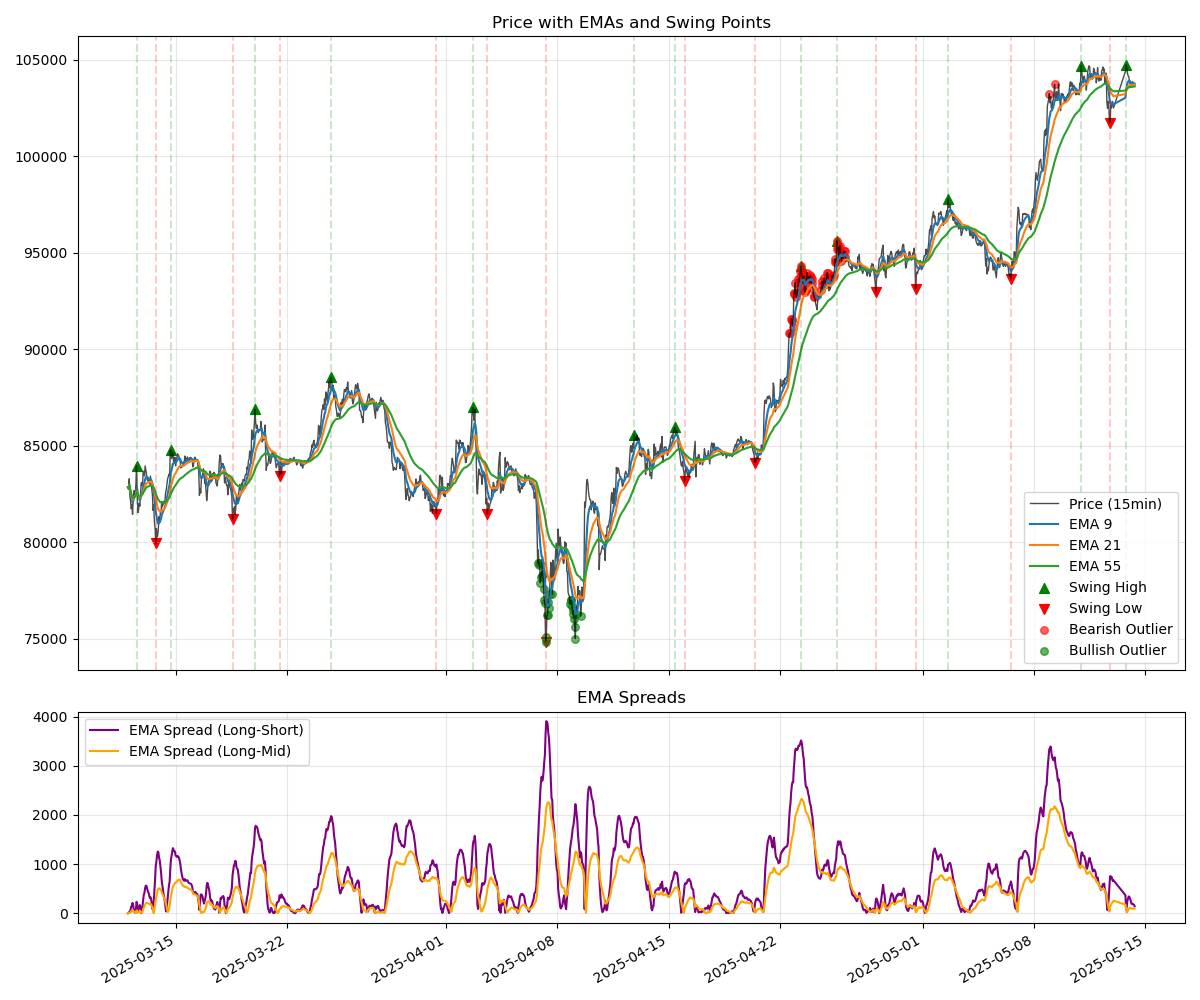
\includegraphics[width=\textwidth]{imgs/swingpoints_emaspread_priceOutliers.png}
    \caption{combined indicators png}
\end{figure}

\footnote{Chart made with Matplotlib and Seaborn}






\newpage
\section{From outliers to strategy}
\subsection{Progress description}
I had a pretty hard time going from developing a logic for the outliers of the Delta. Finding that volatility increases after outliers was a good first find which didn't take long and the process was pretty straight forward. But finding some defenition condtion is meet directional bias was very difficult. By directional bias I mean a price direction which is not random after some kind of condition. It was pretty clear from the begging on that the outliers by there selfe won't offer any kind of directional bias


An outlier is defined as:

\begin{itemize}
  \item \eqref{eq: outlier_detection}.
  $\Delta < \mu(\Delta) - 2\sigma(\Delta) \quad \text{or} \quad \Delta > \mu(\Delta) + 2\sigma(\Delta)    $
\end{itemize}


Then since Bitcoin clearly is not a stationary asset I needed to find some kind of trend identification. I found that the swing points are a good indicator for this.
We determined a trend by using looking at swingpoints. A swing point is a local extrema of a certain period.

\subsection{Where did I start my research}
\begin{verbatim}
  #compute swing points
  swing_points = swing_points(df['price'], period=n)

\end{verbatim}

Parameters of the swing\textunderscore points function:
\begin{itemize}
  \item $n$ is the lookback period
  \item $df['price']$ is the price column of the dataframe (Which is a timeseries)
  \item $P_t$ is a value of $df['price']$ at time $t$
\end{itemize}


We basically got through the time series dataset and look back $n$ $P_t$ values. The highest and lowest points inside of that specific lookback period are the swing points. After that we detetermine if price is making higher highs or lower lows. We check this by storeing the last swing points and wait till we are eighter making a higher high or a lower low.



\subsection{Finding an edge}

\begin{figure}[H]
  \centering
  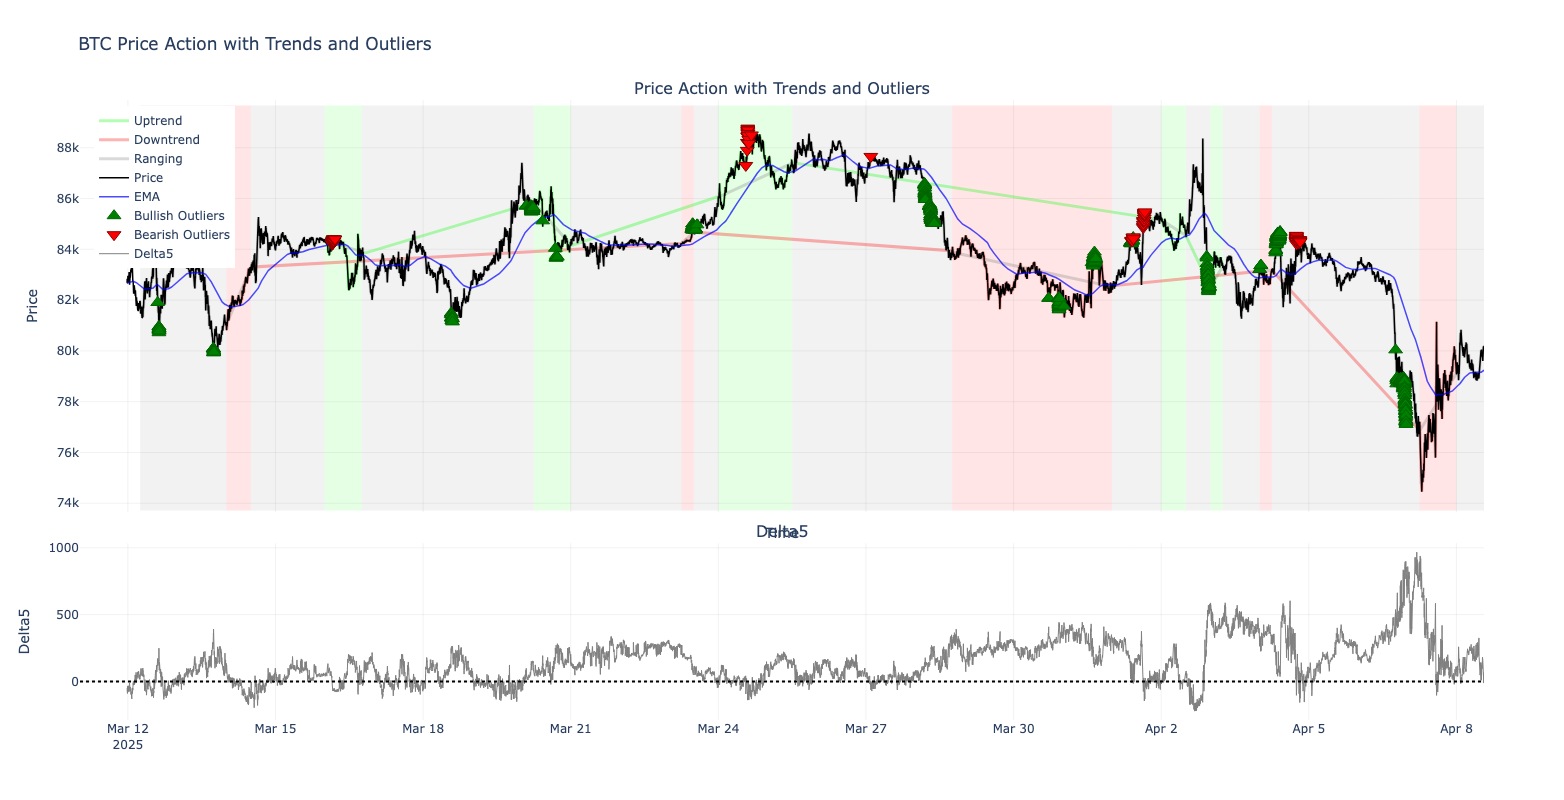
\includegraphics[width=\textwidth]{imgs/plotting_of_my_idea.png}
  \caption{Visualization of $\Delta_t$ outliers and regime identification}
\end{figure}
\begin{figure}[H]
  \centering
  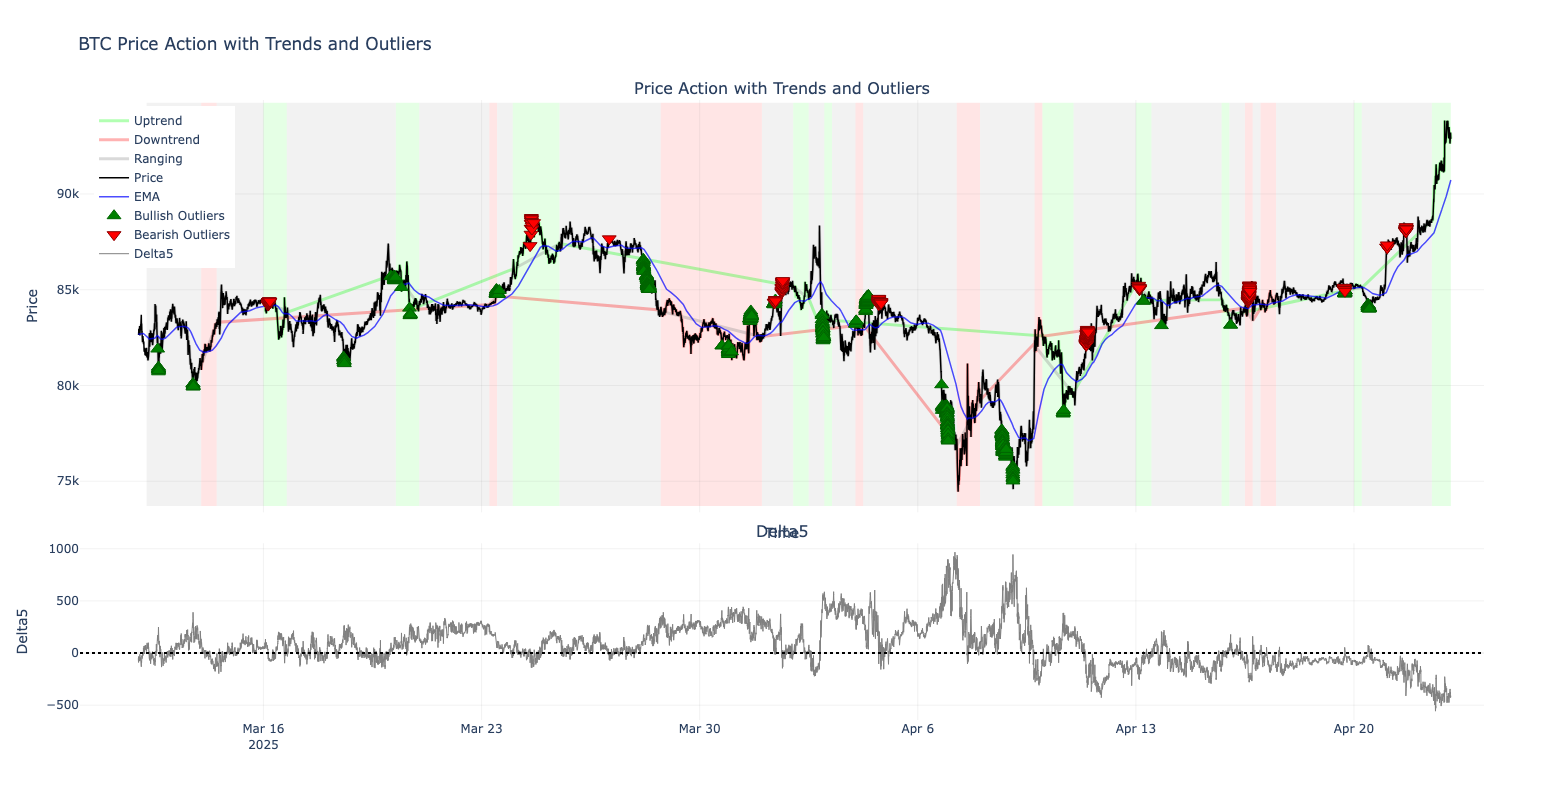
\includegraphics[width=\textwidth]{imgs/v2_plotting my idea.png}
  \caption{Visualization of $\Delta_t$ outliers and regime identification}
\end{figure}

Here you can see two visulaisations of outliers and regime identification. On two different timeseries datasets. This was my trend identification system $v1$ which is only based on swing point mapping.






After plotting different kind of parts of Timeseries Data sets I created I was pretty sure that somewhere I would be finding an edge since the outliers often where at good entry points for a strategy. Only problem was I wasn't able to get any statistical proof ot this.
After finding a Github Repo which used Vectorbt to test 1000 strategies at the same time I tried a similar approach and tested different conditions to see if there was some kind of edge.









\subsection{Monte Carlo Testing}

First of I have to explain how I search for a strategy and how it nearly killed my computer. 
We start by defining a different kind of sample sizes of all the $\Delta_t$ outliers time periods after the outlier detection.


We want to know the return after our condition meets and then check in after $z$ minutes after that
\begin{verbatim}
  sampling_percentages = [0.1, 0.2, 0.6, 0.8, 1.0]
  holding_periods = [60, 120, 240, 360]  
\end{verbatim}

The sampling percentage definies how many of the existing outliers we use and test the returns on. So let's say we have $x$ amount of $\Delta_t$ Outliers. We then randomly select $z$ \% amount of outliers and test the returns on them. We do this 1000 times and then take the average return of all the 1000 tests.
The second step is to test each sampling percentage on the different holding periods. So let's say we have a sampling percentage of $z$ \% and a holding period of $y$ minutes. We then take the $z$ \% amount of outliers and test the returns on them after $y$ minutes. This test is basically copied from the Vectorbt Github Respository. I just changed the code to fit my needs and added some extra information returns. My code gives back the average return, the Sharpe, expectancy and mean Z-Score.

\begin{itemize}
  \item \textbf{Sharpe Ratio}: The Sharpe ratio is a measure of the risk-adjusted return of a strategy. It is calculated by dividing the average return of the strategy by the standard deviation of the returns.
  \item Calculated by $\frac{\overline{r}}{\sigma}$ Where $\overline{r}$ is the average return and $\sigma$ is the standard deviation of the returns.
  \item \textbf{Expectancy}: The expectancy is a measure of the profitability of a strategy. It is calculated by dividing the average return of the strategy by the average loss of the strategy.
  \item Calculated by $\frac{\overline{r}}{\overline{l}}$ Where $\overline{r}$ is the average return and $\overline{l}$ is the average loss.
  \item \textbf{Mean Z-Score}: The mean Z-Score is a measure of the average Z-Score of the strategy. It is calculated by taking the average of the Z-Scores of the strategy.
  \item Calculated by $\frac{1}{n}\sum_{i=1}^{n} z_i$ Where $z_i$ is the Z-Score of the strategy at time $i$ and $n$ is the number of Z-Scores.
  \item \textbf{Average Return}: The average return is a measure of the average return of the strategy. It is calculated by taking the average of the returns of the strategy.
  \item Calculated by $\frac{1}{n}\sum_{i=1}^{n} r_i$ Where $r_i$ is the return of the strategy at time $i$ and $n$ is the number of returns.



\end{itemize}



Now it is time to test some strategies. The first strategy I want to test is pretty intuitive. Measure the average return of bullish outliers inside of an uptrend.

\begin{list}{label}{spacing}
  \item A outlier is bullish if the the orderbook $\Delta_t$ is two standard deviations above the mean of the last 1440 $\Delta_t$ values and bearish if it is two standard deviations below the mean of the last 1440 $\Delta_t$ values.

\end{list}

Now when we backtest a strategy we have to have a few things in mind. First of all we are backtesting on on historical data and if we just use different kind of entry conditions we might just change the entry conditions till we have a good end results. This would be overfitting and not work on future data. 
In order to prevent overfitting we have to use a holdout sample. I have one dataset on which we test our entry conditions to see if they even have potential. 





If these conditions are met for a condition I test on some out of sample data. (Out of sample data just means that we test on new data)
Most of the time things end up not even passing the first out of sample test and lose their potential instantly. If not I have another out of sample test and if that one is passed we are ready to do some more monte carlo testing and look how potential equity curves look like.
And to make things even worse we can assume that the sharpen ratio will decrease by atleast 20\% compared to the backtest simulation.




\newpage


\subsection{Backtesting framework}

My backtesting framework is built in Python using the VectorBT library and consists of several key components:

\subsubsection*{Data Pipeline}

Connection to Postgres database hosted on railway.app with global access. \href{https://customchart-production.up.railway.app/#}{Live data mining progress}
\begin{itemize}
  \item Historical price data from Coinbase (BTC/USD)
  \item Orderbook delta data at different depths ($\Delta_{1\%}$, $\Delta_{2.5\%}$, $\Delta_{5\%}$)
  \item 1-minute timeframe for base calculations
  \item Direct ema calculation which a lenght of 50 on the 1h timeframe
\end{itemize}





\subsubsection*{Testing Methodology}
The framework implements a three-stage testing process:
\begin{enumerate}
  \item \textbf{Initial Sample Testing}
    \begin{itemize}
      \item Test strategy on initial dataset
      \item Multiple sampling percentages: [0.1, 0.2, 0.6, 0.8, 1.0]
      \item Various holding periods: [60, 120, 240, 360] minutes
    \end{itemize}
  
  \item \textbf{Out-of-Sample Validation}
    \begin{itemize}
      \item Test promising strategies on separate dataset (Two different datasets)
      \item Require consistent performance across datasets
    \end{itemize}
  
  \item \textbf{Monte Carlo Simulation}
    \begin{itemize}
      \item Random sampling of trade opportunities
      \item 1000 iterations per test configuration
      \item Analysis of distribution of outcomes
    \end{itemize}
\end{enumerate}

\subsubsection*{Performance Metrics}
Each strategy is evaluated using:
\begin{itemize}
  \item \textbf{Sharpe Ratio}: $\frac{\overline{r}}{\sigma}$
  \item \textbf{Expectancy}: $\frac{\overline{r}}{\overline{l}}$
  \item \textbf{Average Return}: $\frac{1}{n}\sum_{i=1}^{n} r_i$
\end{itemize}

\subsubsection*{Risk Management}
The framework incorporates:
\begin{itemize}
  \item Trading fees (0.003\% on Hyperliquid)
  \item  Slippage of (0.0001\% on Hyperliquid)
  \item Maximum drawdown limits
  \item Stop-loss and take-profit levels
\end{itemize}

\subsubsection*{Implementation}
\begin{verbatim}
# Example of strategy implementation
def backtest_strategy(data, params):
    # Define entry/exit signals
    outlier_mask = (data['outlier_context'] == 's') & 
                   (data['trend'] == 'Uptrend')
    
    # Create portfolio simulation
    pf = vbt.Portfolio.from_signals(
        close=data['price'],
        entries=outlier_mask,
        exits=exits_after_n_bars(outlier_mask, n=params['holding_period']),
        init_cash=100,
        freq='1T'
    )
    
    return calculate_metrics(pf)
\end{verbatim}

This framework allows for rapid testing of multiple strategy variations while maintaining strict validation criteria to prevent overfitting.












\newpage
\section{Developing a strategy}

\subsection{Initial thoughts}

I will only able to show a few strategies backtests since I tested on about 150 different logics and only 1 of them passed all the out of sample tests. I will show the best ideas I had and the results of the backtests.


\subsection{Reverse strategy}
So logical thinking we could assume that long strategy can be reversed into a short strategy and vice versa. The problem is that we have fees and slippage. So we need a certain amount of profit to cover the fees and slippage. And since my strategy has a rather high frequency we need to have a lot of trades to cover the fees and slippage.




\subsection{First strategy test}
So the first strategy I test was before I developed the backtesting framework. I was testing on a simple logic. If the price on the 1h timeframe closed above the 50 period EMA and the $\Delta_5$ of the orderbook was positive we would enter a buy position if price was in a range of $0.05\%$ of the $EMA_50$.


In addition to that I was using a trailing stop. The trailing stop was set to $1\%$ of the price.
A trailing stop is a stop loss that is adjusted to the price of the asset. So if the price goes up the stop loss goes up with it. The idea behing this is that we can catch a bigger upwards in contrast to a fixed stop profit.

I only tested this on a short sample of data because I just had started my data mining process and didn't have any more data. But I can asure that more data didn't make it more profitable just worse.


\subsubsection{Code}

\begin{verbatim}
  # Define entry/exit signals
  range_pct = 0.0005
  trailing_stop_pct = 0.01

  entries = (
    (df['bias'] > df['ema']) &
    (df['price'] >= df['ema'] * (1 - range_pct)) &
    (df['price'] <= df['ema'] * (1 + range_pct))
  )

\end{verbatim}

\subsubsection{Strategy 1 results}

\begin{table}[H]
  \centering
  \caption{Detailed backtest results for the first strategy test.}
  \label{tab:strategy_1_detailed_results}
  \small
  \begin{tabular}{@{}lr@{}}
    \toprule
    \textbf{Metric} & \textbf{Value} \\
    \midrule
    \multicolumn{2}{c}{\textbf{General}} \\
    \midrule
    Start                         & 2025-03-12 00:00:01 \\
    End                           & 2025-03-17 07:24:01 \\
    Period (minutes)              & 7,636 \\
    \midrule
    \multicolumn{2}{c}{\textbf{Performance}} \\
    \midrule
    Start Value                   & 100.00 \\
    End Value                     & 97.13 \\
    Total Return [\%]             & -2.87 \\
    Benchmark Return [\%]         & 0.38 \\
    Total Fees Paid               & 2.21 \\
    Open Trade PnL                & 0.23 \\
    \midrule
    
    

    \multicolumn{2}{c}{\textbf{Trades}} \\
    \midrule
    Total Trades                  & 23 \\
    Closed Trades                 & 22 \\
    Win Rate [\%]                 & 31.82 \\
    Profit Factor                 & 0.75 \\
    Expectancy                    & -0.14 \\
    Best Trade [\%]               & 3.15 \\
    Worst Trade [\%]              & -1.24 \\
    Avg Winning Trade [\%]        & 1.35 \\
    Avg Losing Trade [\%]         & -0.83 \\
    
    \bottomrule
  \end{tabular}
\end{table}

\subsection{Learning from the first strategy}
So from march till july I didn't backtest any strategies. I was focusing on developing signals and indicators. This backtest clearly showed me that I have to do research first and have some kind of background idea of what I am doing.


\newpage

\subsection{Explaining figure}
So on the $Y$ axis we have the average return of the strategy. And on the $X$ axis we have the sampling percentage. 
A sampling percentage of 10\% means that we are using 10 random precentage of the $\Delta_t$ outliers my system identified over the backtesting timeseries dataset and then testing the returns on them. We conduct this 1000 times and then take the average return of all the 1000 tests. In addition to that we are testing the returns on different holding periods. So for example if we are testing the returns on a holding period of 60 minutes we are testing the returns on the 10 random precentage of the outliers after 60 minutes. We conduct this 1000 times and then take the average return of all the 1000 tests.




\begin{figure}[H]
  \centering
  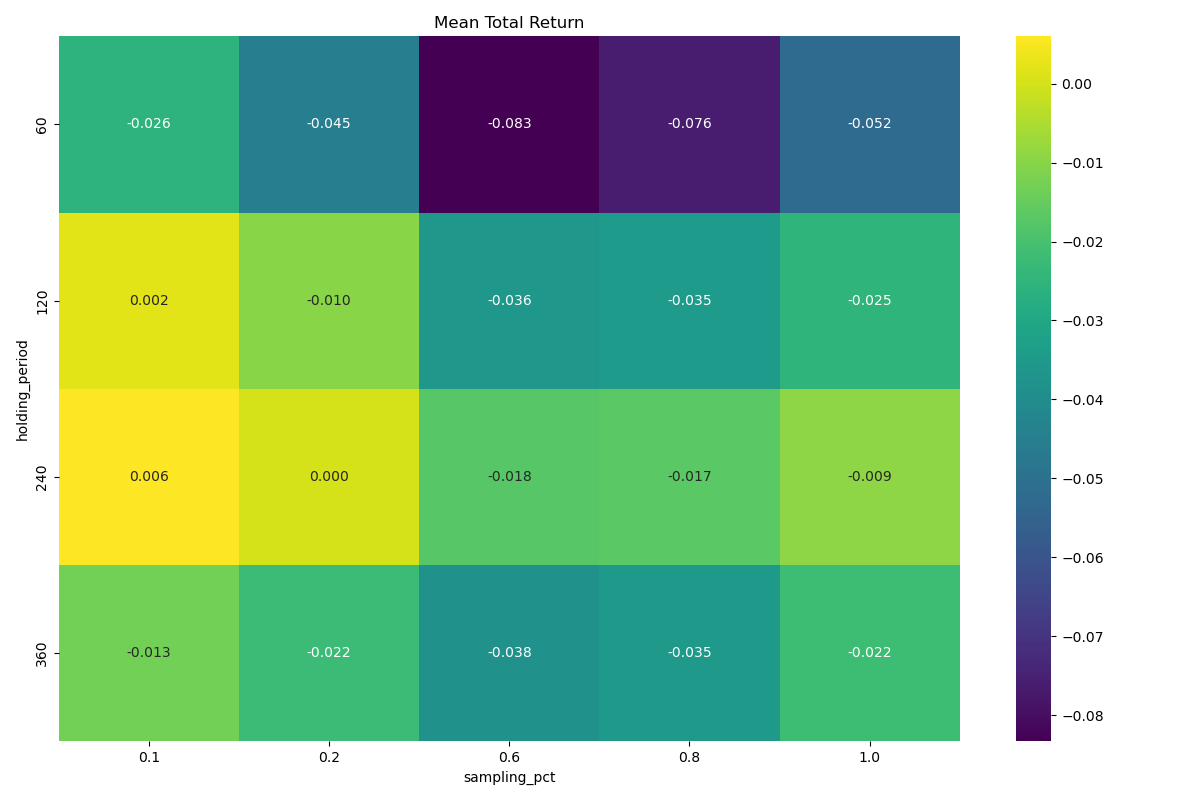
\includegraphics[width=\textwidth]{imgs/Bullish_outliers_inside_of_uptrend.png}
  \caption{Strategy 2 results}
  \label{fig:bullish_outliers_inside_of_uptrend}
\end{figure}


\subsection{Strategy 2}

So this was the second strategy I tested and the first time I used my new backtesting framework. 
Results from this backtest: \ref{fig:bullish_outliers_inside_of_uptrend}

\begin{itemize}
  \item  A $\Delta_{5,t}$ value is identified as a bullish outlier (see Section~\ref{sec:outlier_detection}).
  \item Trend is identified as uptrend
\end{itemize}












\newpage
\section{sources}
{\small
\subsection{\href{https://x.com/HangukQuant/status/1930603876069335120}{How good or random is your trading}}
Twitter article about random walk theory and how to test if a strategy is random or not. 
%\subsection{\href{https://github.com/polakowo/vectorbt}{Testing 1000 strategies at the same time (via Monte Carlo)}}
\subsection{\href{https://x.com/abetrade/status/1941613701150188008}{Tweets}}
A lot of my ideas come from thiy guys Tweets, to research into this. He is a disgresionary trade what means he trades based on his own decisions and has a mental framework to trade. I learned what an orderbook delta is from him.
\subsection{\href{https://trdr.io/}{TRDR} This platform allow you to use different kind of metrics on different Timeseries datasets (BTC/USD Price, orderbookdelta  and Open Interest}his platform allow you to use different kind of metrics on different Timeseries datasets like: BTC/USD Price orderbookdelta  and Open Interest
\subsection{\href{https://github.com/neurotrader888/TrendLineAutomation}{Trend line automation}} Used this for the $v3$ version of my trend identification system
\subsection{\href{https://github.com/polakowo/vectorbt}{Vectorbt github documentation respository.}} I implemented some ideas from this repository for my backtesting framework and used vectorbt for the fees and slippage implementations


\subsection{\href{https://github.com/AJslashTracey/deep_research_chatGPT_03}{Deep research by ChatGPT}}
The OpenAI subscription enables you use deepsearch function from chatGPT I would say this tool is probably useful for research but I didn't find any value from this besides finding out about new indicators. The only thing finding I made from these two pdfs was the Aroon indicator which I implemented in the second verions of my trend indentification system $v2$


\subsection{\href{https://www.r-5.org/files/books/trading/charts/market-profile/James_Dalton-Markets_in_Profile-EN.pdf}{Markets in profile -- James Dalton}}
Altho this book is for a disgresionary trading approach it taught me a lot about the Efficient Market Hypothesis and trading psychology.

\subsection{\href{https://x.com/i/grok/share/q9fAogSBPA92zR0lgXd4q9OZT}{Do retail traders stande a chance?}}

Good read about if retail traders even have a chance to beat the market.
}


\end{document}